\documentclass{../../text-style}

\texttitle{Веб-программирование, часть 1}

\begin{document}

\maketitle
\thispagestyle{empty}

\section{Введение}

Эпоха десктопных и тем более консольных приложений постепенно подходит к концу. Большинство современных систем распределённые и имеют веб-фронтенд, и с развитием веб-технологий веб-приложения используются даже в областях, традиционных для десктопных приложений --- например, появляются веб-IDE с облачной компиляцией, веб-графические редакторы, веб-UML-рисовалки и т.д. и т.п. Не говоря уже об информационных системах, на долю которых приходится большинство разрабатываемого в мире софта --- хоть они и используются, как правило, в рамках только одной организации, веб-интерфейс считается чем-то самим собой разумеющимся. Более того, некоторые приложения выдают себя за десктопные, но на самом деле представляют собой урезанный браузер, показывающий HTML-разметку и исполняющий обычный JavaScript (например, Discord, Steam, даже MS Teams и Visual Studio Code). В общем случае это не очень хорошая идея, поскольку нативные библиотеки часто работают в разы быстрее, но вот VS Code неплохо получился в плане скорости работы (возможно, это как-то связано с тем, что фреймворк WPF\footnote{Windows Presentation Foundation}, стандарт де-факто для разработки десктопных приложений под Windows, каким-то образом даже медленнее, чем JS + HTML в браузере).

К несчастью, веб-разработка --- это отдельный мир, со своими технологическими стеками (причём их тысячи), миллионом разных задач и миллионом разных решений, которые при этом ещё и постоянно меняются, появляются новые и выходят из моды старые. Так что сегодня речь пойдёт про то, как всё в целом работает внутри, плюс про то, как это работает конкретно на .NET, в этой лекции --- со стороны сервера (хотя чуть-чуть про фронтенд всё-таки будет, куда же без него). Но надо понимать, что все технические подробности, изложенные тут, \emph{уже} устарели. Мир веб-разработки вообще отличается тем, что раз в год-два меняется до неузнаваемости. Но если понимать основные принципы, разобраться в деталях нового JS-фреймворка проблем не составит.

Итак, как вообще работают веб-приложения:

\begin{itemize}
    \item Пользователь заходит браузером на определённый URL. На самом деле, браузер при этом выполняет HTTP GET-запрос на порт 443 или 80 (443 --- если протокол HTTPS, в современных интернетах почти всегда используется именно он; 80 --- если HTTP). При этом сначала парсится URL, выполняются DNS-запросы и т.д., как рассказывалось в лекции про сети.
    \item ОС сервера перенаправляет запрос запущенному там \emph{веб-серверу} --- например, Apache или IIS. Также с ростом популярности Docker и контейнеризации нынче популярны \emph{self-hosted} сервисы, например, Kestrel --- каждое веб-приложение поднимает свой мини-сервер, который обслуживает только его. Это позволяет приложению ни от чего не зависеть и запускаться одной командой даже на <<голой>> машине без всего.
    \item Веб-сервер --- отдельный процесс, в рамках которого запущено одно или несколько \emph{веб-приложений}, веб-сервер по URL запроса определяет, какому веб-приложению он адресован, и передаёт запрос ему.
    \item Веб-приложение построено на базе какого-нибудь \emph{веб-фреймворка}, который выполняет всякие инфраструктурные вещи типа парсинга параметров запроса, проверки аутентификации и авторизации, и т.д. В конечном итоге фреймворк с помощью пользовательского кода формирует ответ и отправляет его обратно по HTTP в виде HTML-страницы.
    \item Эта страница и показывается пользователю в браузере. В современном мире <<страница>>, как правило, состоит из кучи JavaScript-кода, который исполняется в браузере независимо, посылает при необходимости асинхронные запросы на сервер, и может хоть полностью перестраивать HTML в зависимости от действий пользователя.
\end{itemize}

А ещё есть \emph{веб-сервисы}, которые похожи на веб-приложения, но предназначены не для людей и браузеров, а для других приложений (в том числе, специально чтобы всех запутать, веб-сервисы часто обслуживают запросы от браузерных клиентов, работающих на JavaScript). Только самые маленькие современные веб-приложения --- это фронтенд и бэкенд, приложения побольше состоят из нескольких отдельных веб-сервисов, которые совместно исполняют запрос, общаясь по сети друг с другом. Они уже не используют HTML, хотя так же, как обычные веб-приложения, используют HTTP/HTTPS как транспортный протокол. Пример специфичного для веб-сервисов протокола --- SOAP (ранее известный как Simple Object Access Protocol), фактически протокол удалённого вызова методов у объектов. SOAP предполагает обмен по HTTPS XML-пакетами с сериализованными именами методов, их параметрами и результатами вызова. Помимо SOAP ещё популярен gRPC (то же самое по сути, но попроще, побыстрее и с бинарным протоколом сериализации, а не XML). Есть ещё REST, про который многие неправильно думают, что это протокол, но на самом деле это архитектура построения приложений на веб-сервисах, описывающая в том числе и соглашения по передаче данных. Не настолько подробно, чтобы это можно было назвать протоколом, но он достаточно много специфицирует --- запрет на хранение информации о конкретном подключении, например.

Технологии для создания веб-сервисов обычно также содержат механизмы для публикации метаинформации о сервисе, в частности, какие методы он содержит, какого типа у них параметры, что они возвращают. Метаинформация предоставляется в машиночитаемом виде, и её обычно достаточно, чтобы автоматически сгенерировать клиентскую \emph{заглушку} (на самом деле, прокси) --- класс, который выглядит, как обычный класс с методами как у веб-сервиса, но сам ничего не делает, а просто пересылает вызовы сервису и десериализует результат. Так что использование веб-сервиса в приложении --- задача совсем несложная (и на самом деле даже без заглушки запросы пишутся обычно весьма прямолинейно --- см., например, VK API). Для SOAP-сервисов метаинформация публикуется по протоколу WSDL\footnote{Web Service Description Language}, часто она доступна для скачивания по адресу, похожему на адрес сервера (что-то вроде \url{https://example.com/my_service/wsdl}). Для gRPC это .proto-файлы, они не публикуются стандартным образом, но часто выкладываются в открытый доступ, для REST --- это OpenAPI-спецификация, генерируемая и публикуемая инструментом Swagger.

Разработка веб-сервисов --- это отдельное поднаправление в мире веб-разработки. Тут тоже есть свои технологические стеки. В .NET, например, для этого может использоваться ASP.NET Web APIs (часть ASP.NET, про которую будет дальше), также популярна gRPC, в корпоративных системах всё ещё массово используется WCF\footnote{Windows Communication Foundation}, на базе которой во многом и написан ASP.NET (и призван её заменить, так что новые приложения на WCF уже не надо делать). В Java-мире это в основном библиотека Spring.

Вот краткий обзор технологического стека для .NET веб-приложений или веб-сервисов. Однако надо понимать, что в принципе все технологии одного предназначения весьма взаимозаменяемы и если, например, Microsoft поставляет свою СУБД (MS SQL Server), это не значит, что веб-приложения под .NET будут работать только с ней. На самом деле, с ней как раз мало кто работает в силу наличия бесплатных и достаточно хороших СУБД, либо платных, но более производительных.

\begin{itemize}
    \item Веб-сервер --- IIS\footnote{Internet Information Services}, IIS Express, Kestrel. IIS ставится прямо с Windows (правда, его там надо включить и настроить, и далеко не факт, что он будет работать в Home Edition), IIS Express поставляется в комплекте с Visual Studio и запускается сам, ничего скачивать и настраивать не нужно. Но полезен он только для отладки. Kestrel ставится как библиотека в составе ASP.NET, тоже не требует особой настройки и может работать и в production-окружении (и обычно нынче используется как раз он, потому как задачи, решаемые IIS, типа управления жизненным циклом веб-приложения, решает Docker, точнее Docker Compose).
    \item Технология для разработки веб-приложений и веб-сервисов --- ASP.NET. Именно на её примере будет дальнейший рассказ.
    \item СУБД --- MS SQL Server (платный) или SQL Server Express (бесплатный, но с ограничениями). Особенно интересен SQL Server Express LocalDB --- СУБД, позволяющая только локальные подключения, но очень легковесная и простая в настройке. Вообще, выбор СУБД для веб-приложений очень богат: LocalDB хороший вариант на начальных этапах, затем можно перейти на MariaDB или PostgreSQL, или вообще сразу использовать что-то из NoSQL-СУБД, например, MongoDB. Зачем вообще веб-приложениям базы данных --- дело в том, что приложение может быть остановлено после обработки \emph{каждого} запроса, как решит веб-сервер. И запущено заново при поступлении нового запроса. Поэтому хранить данные в памяти попросту бесполезно, базы данных попросту обязательны, если ваше веб-приложение работает с информацией, которую можно изменять.
    \item Если вы выбрали реляционную СУБД, вам потребуется ещё ORM\footnote{Object-Relational Mapping}-система. В мире .NET это прежде всего Entity Framework (нынче Entity Framework Core), хотя есть и альтернативы (например, NHibernate --- переписанный под .NET фреймворк Hibernate, стандарт де-факто для ORM в мире Java).
    \item Фронтенд, как обычно, пишется на HTML + JavaScript, но постепенно <<сырой>> JavaScript становится дурным тоном. В индустрии его потихоньку вытесняет TypeScript --- язык от Microsoft, который по сути компилируемая типизированная надстройка над JavaScript. Не то чтобы напрямую относится к стеку технологий .NET, на TypeScript прекрасно можно писать без всякого .NET (он использует JS-стек, вокруг NPM\footnote{Node Package Manager} в основном), но мало какое веб-приложение в современном мире без него обходится.
    \item Написанное приложение надо как-то деплоить, причём у веб-приложений обычно куча зависимостей и куча опций настройки, причём, поскольку веб-приложения не надо переустанавливать конечным пользователям, деплой часто выполняется после каждого коммита (по нескольку раз \emph{в день}). Чтобы это не превращалось в кошмар, веб-приложения упаковывают в Docker-контейнеры --- по сути, маленькие и быстрые виртуальные машины для одного процесса, где есть само приложение, и вообще всё, что нужно ему для работы. Как ни странно, .NET-приложения чаще всего упаковывают в Linux-контейнеры и запускают на Linux-машинах, даже в Microsoft-овской инфраструктуре, для этого в Windows даже относительно недавно сделали поддержку ядра Linux --- WSL\footnote{Windows Subsystem for Linux}. Это настоящее ядро Linux, работающее на мини-виртуалке и способное исполнять линуксовые программы.
    \item Даже когда мы собрали контейнер с нашим приложением, его надо задеплоить на каком-то \emph{хостинге}. Поставить в угол компьютер с IIS и запустить приложение там --- плохая идея, потому что выключат интернет (или электричество), и приложение помрёт. У Microsoft есть свой облачный хостинговый сервис (на самом деле, не хостинг, а целая инфраструктура, включающая в себя и машины для запуска Docker-контейнеров, и отдельные СУБД, которые никуда ставить не надо, и ещё кучу всего) --- Azure. Как обычно, есть и альтернативы --- прежде всего, Amazon, ещё Heroku, Яндекс.Облако (если не хотите нарваться на проблемы с российским законодательством, запрещающим, в частности, хранить персональные данные не на территории России). Azure имеет бесплатный план, достаточно хорош и хорошо интегрирован с IDE от Microsoft, но Amazon принадлежит что-то около 80 процентов рынка облачной инфраструктуры...
\end{itemize}

Итак, жизненный цикл разработки типичного небольшого веб-приложения примерно такой:

\begin{itemize}
    \item определяемся, надо ли нам хранить данные и обеспечивать коллаборативную работу --- если нет, то, скорее всего, можно обойтись чисто клиентским веб-приложением, без серверной части; это предпочитаемый вариант, потому что такие приложения гораздо проще хостить;
    \item если всё-таки надо, нам потребуется серверная часть; сначала понимаем, какие запросы будут к нашему веб-приложению (HTML-страницы и запросы к API), пишем контроллеры (про них чуть попозже) и серверную логику;
    \item примерно в это время будет понятно, какие данные надо хранить, описываем схему БД (можно прямо в коде --- подходом Code First), настраиваем СУБД и ORM-систему;
    \item набрасываем вёрстку фронтенда (того, что будет работать в браузере) на HTML с какой-либо библиотекой стилей (Bootstrap, например), говорим методам контроллеров возвращать эти страницы; можно сразу верстать с помощью какой-нибудь высокоуровневой фронтенд-библиотеки, например, React, но сразу потребуется сделать следующий шаг;
    \item пишем клиентскую логику --- настраиваем компиляцию TypeScript, пишем скрипты, что-то делающие с HTML, подключаем их к свёрстанным ранее HTML-страницам, проверяем всё в сборе;
    \item настраиваем упаковку в Docker-контейнер (и, желательно, сборку прямо в контейнере, чтобы не зависеть от версий инструментов разработки); если требуется несколько сервисов (включая, возможно, сторонние, типа СУБД) --- настраиваем Docker Compose;
    \item запускаем всё локально из контейнеров (в идеале --- командой docker-compose up), заходим браузером на правильный порт, проверяем, что всё работает;
    \item настраиваем облачное окружение, например, на Azure, деплоим контейнеры туда;
    \item идём на выданный нашему приложению Azure URL, проверяем, что всё работает и там;
    \item повторяем все предыдущие шаги до тех пор, пока не окажемся удовлетворены результатом.
\end{itemize}

Теперь поговорим подробнее об этих этапах, и начнём с фронтенда, потому что для многих приложений им же можно и закончить. В этой лекции будут самый минимум про фронтенд, в следующей поговорим и про клиентские библиотеки.

\section{Фронтенд}

Клиентская часть веб-приложений исполняется в браузере у пользователя. Современный браузер по сути --- виртуальная машина, которая умеет \emph{рендерить} HTML-документы и исполнять код на JavaScript, который позволяет ими манипулировать. 

HTML\footnote{HyperText Markup Language, если кто не в курсе} используется для задания содержимого и структуры отображаемого документа, не внешнего вида (так что если вас где-то учили атрибутам типа color у HTML-тэгов, забудьте про них навсегда). Самый полезный в плане разметки HTML-тэг --- это \mintinline{html}{<div>}, описывающий просто раздел документа, без какого-либо его визуального оформления. Однако активно используются и параграфы, заголовки, списки, таблицы и т.д. и т.п. (так называемая <<семантическая вёрстка>>, разметка документа исходя из его структуры). На <<структурные>> тэги также навешиваются атрибуты для их идентификации --- id и, при необходимости, class, чтобы их было проще искать в скриптах и в стилях. Причём id бывают автогенерённые, что не очень хорошо, потому что для работы с тэгами из скриптов их стоит называть как-то мнемонично.

Внешний вид страницы определяется отдельно в виде CSS\footnote{Cascading Style Sheet}-документа. Там как раз и выставляются атрибуты внешнего вида для целых классов элементов, хотя их можно указать и для конкретного элемента с конкретным id-шником. Атрибуты включают в себя в том числе и расположение элемента на странице, поэтому поменяв CSS, можно полностью изменить внешний вид страницы. К счастью, есть распространённые библиотеки стилей (например, Bootstrap), которые содержат готовые CSS-ки, заставляющие любую страницу выглядеть пристойно (если вы правильно разметите атрибуты class у тэгов).

Ну и последний элемент мозаики --- JavaScript. Это вполне себе работоспособный язык программирования, скрипты на котором качаются вместе со страницей и интерпретируются браузером. Относиться к нему, однако, стоит как к ассемблеру (или, точнее, IL-коду) --- писать на JavaScript можно, но это не приносит радости, и даже если вы на нём пишете, браузер, скорее всего, исполняет не прямо ваш код. В реальных проектах используются различные транспиляторы и минимизаторы, которые берут человекочитаемый код и переводят на другую версию языка, чтобы его поняли даже старые браузеры, или заменяют названия переменных на a, b, c и т.п. и выкидывают переводы строк --- потому что браузеру для исполнения это не надо, а объём передаваемых по сети данных несколько уменьшит. Поскольку для JavaScript есть куча довольно больших библиотек, и любое нормальное веб-приложение использует их сотни (считая со всеми зависимостями, конечно), минимизация довольно критична в плане скорости загрузки страницы.

\subsection{Document Object Model}

DOM (Document Object Model) --- это представление HTML-документа в виде дерева объектов и API для доступа к нему. Браузер парсит присланный HTML-документ и строит по нему DOM, по окоторому потом можно ходить скриптами или делать запросы через CSS-селекторы (о которых чуть попозже) или запросы XPath. API позволяет как читать, так и произвольно редактировать дерево --- добавлять, удалять элементы, менять атрибуты и т.д. Браузер перерисовывает страницу каждый раз, когда DOM меняется, что и даёт возможность делать интерактивные веб-приложения.

Например, если есть такой фрагмент HTML-документа:

\begin{minted}{html}
<table class="listing">
    <thead>
        <tr class="odd">
            <th>Выпускник</th>
            <th>Научный руководитель</th>
            <th>Текст</th>
        </tr>
    </thead>
    <tbody>
        <tr class="odd">
            <td>Акбаров Артур Александрович</td>
            <td>д.т.н., проф. Д.В. Кознов</td>
            <td><a href="bmo/441-Akbarov-report.pdf">Текст</a></td>
        </tr>
    </tbody>
</table>
\end{minted}

То соответствующее ему DOM-дерево может выглядеть как-то так:

\begin{center}
    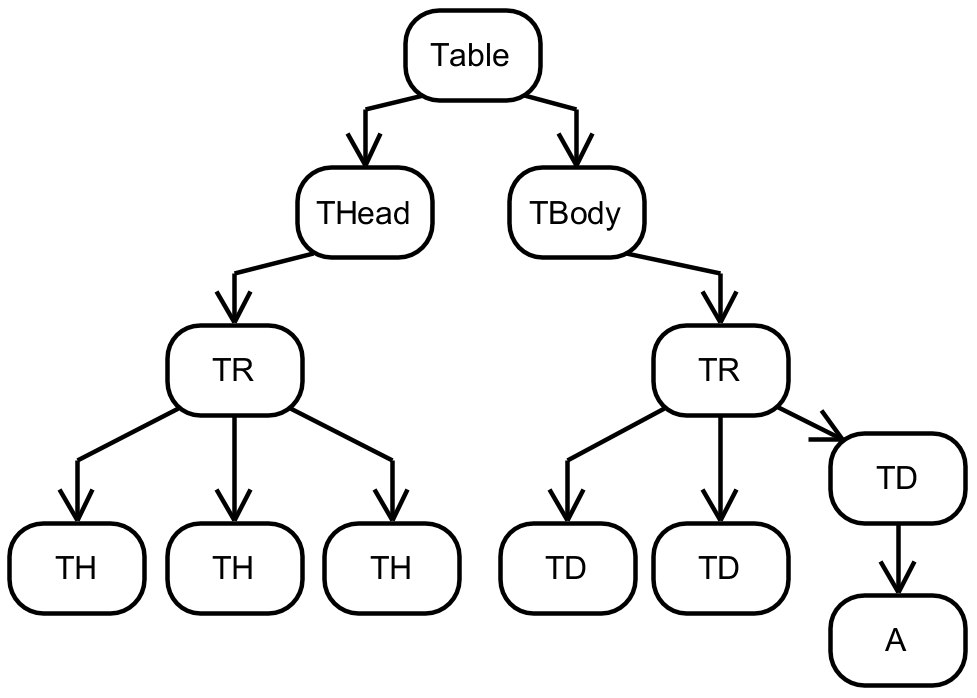
\includegraphics[width=0.5\textwidth]{domTree.png}
\end{center}

\subsection{HTML-формы}

Если надо что-то отправить обратно на сервер, то есть два варианта --- асинхронный запрос из JavaScript (AJAX-запрос, про них чуть позже), либо стандартными средствами HTML, без JavaScript вовсе --- через HTML-форму. Есть тэг \mintinline{html}{<form>}, дочерними тэгами которого должен быть набор тэгов \mintinline{html}{<input>}, один из которых должен иметь type submit:

\begin{minted}{html}
<form method="post">
    First name:<br>
    <input type="text" name="firstName"><br>
    Last name:<br>
    <input type="text" name="lastName"><br><br>
    <input type="radio" name="gender" value="male" checked>Male<br>
    <input type="radio" name="gender" value="female">Female<br>
    <input type="submit" value="Submit">
</form>
\end{minted}

\mintinline{html}{<input>} --- это то, куда пользователь может вводить данные, он может быть разных типов, например, просто строка, кнопка-переключатель, кнопка-флажок и т.д. Когда пользователь жмёт на \mintinline{html}{<input>} типа submit (который выглядит ка обычная кнопка), данные из полей input, введённые пользователем, (или соответствующие им значения атрибута value) сериализуются и отправляются на сервер в виде, как правило, POST-запроса (хотя можно указать желаемый HTTP-метод как атрибут у формы). Сервер может десериализовать присланные данные и что-то с ними сделать (например, сохранить в базу данных), и в конечном итоге он должен в ответ отправить новую HTML-страницу, которую снова отрендерит браузер. Поэтому формы --- это быстрый и простой, но непопулярный нынче метод отправки пользовательского ввода, потому как требует перезагрузки всей страницы. В современном мире это практикуется, и часто даже уместно, когда грузить новую страницу надо и так: например, после авторизации пользователя. Однако всё чаще общение с сервером происходит незаметно для пользователя и без всяких перезагрузок страницы, асинхронными запросами из JavaScript.

\subsection{CSS}

Cascading Style Sheet --- это правильный способ задать внешний вид HTML-документа. CSS --- это, как правило, отдельный файл, на отдельном языке, где описывается, к каким тэгам надо применить какие атрибуты. Cascading оин неспроста, CSS-ок может быть много и они применяются последовательно, возможно, переопределяя друг друга, так что может быть стиль приложения в целом, который переопределяется стилем всех кнопок, который переопределяется стилем конкретной кнопки. При этом атрибуты просто сваливаются в одну кучу (возможно, переопределяя друг друга) и добавляются к соответствующим тэгам, после чего то, что получилось, уже рендерит браузер. Вот так выглядит HTML-документ со <<встроенным>> CSS-ом\footnote{Тут и ниже примеры из \url{https://www.w3schools.com} (дата обращения: 18.11.2021), незаменимого образовательно-справочного ресурса по всему, что свазано с веб-разработкой.} (не делайте так):

\begin{minted}{html}
<!DOCTYPE html>
<html>
    <head>
        <style>
            body {background-color: powderblue;}
            h1   {color: blue;}
            p    {color: red;}
        </style>
    </head>
    <body>
        <h1>This is a heading</h1>
        <p>This is a paragraph.</p>
    </body>
</html>
\end{minted}

А вот тот же HTML-документ, где CSS вынесен в отдельный файл (делайте так):

\begin{minted}{html}
<!DOCTYPE html>
<html>
    <head>
        <link rel="stylesheet" href="styles.css">
    </head>
    <body>
        <h1>This is a heading</h1>
        <p>This is a paragraph.</p>
    </body>
</html>
\end{minted}

В styles.css --- то самое, что было в тэге style выше.

Что происходит в этом примере:

\begin{itemize}
    \item тэгу body выставляется атрибут background-color, равный powderblue;
    \item всем тэгам h1 выставляется атрибут color, равный blue;
    \item всем тэгам p выставляется атрибут color, равный red.
\end{itemize}

Получается очень психоделично свёрстанная страница, так тоже не делайте.

Более тонко настраивать вид тэгов можно с помощью \emph{CSS-селекторов}, которые позволяют фильтровать тэги по типу (это мы как раз только что видели), классу и id. Например:

\begin{minted}{html}
<p id="p01">I am different</p>
<p class="error">Error message</p>
\end{minted}

И соответствующий CSS:

\begin{minted}{css}
#p01 {
    color: blue;
}

p.error {
    color: red;
}
\end{minted}

Несколько селекторов, если они записаны подряд без разделителей, означают <<и>>. Разделитель-пробел означает <<найди сына>>, например, <<div p>> означает выбрать все элементы p внутри всех элементов типа div (при этом сам div такой селектор не выбирает), разделитель-запатая означает <<или>>, например, <<div,p>> означает <<все тэги div и все тэги p>>. Можно делать выборку по атрибутам, селекторами вида <<[attribute]>> и <<[attribute=value]>>. И ещё много чего можно, это странный, но вполне развитый язык запросов к иерархическим данным. Подробности, как обычно, на сайте W3 Schools: \url{https://www.w3schools.com/cssref/css_selectors.asp}.

\subsection{JavaScript}

Наконец, небольшая ликвидация безграмотности по JavaScript. Поскольку рассказывать про синтаксис и модель исполнения JavaScript нет ни времени, ни нужды, ограничимся парой примеров. Вот что-то в духе "Hello, world":

\begin{minted}{html}
<!DOCTYPE html>
<html>
    <body>

    <h1>My First JavaScript</h1>

    <button type="button"
        onclick="document.getElementById('demo').innerHTML = Date()">
        Click me to display Date and Time.
    </button>

    <p id="demo"></p>

    </body>
</html> 
\end{minted}

Тут мы в качестве значения атрибута onclick у button передаём код на JavaScript, который браузер будет исполнять, как нетрудно догадаться, каждый раз, когда пользователь нажимает на кнопку. В нём мы у глобальной переменной document, представляющей тот самый DOM, о котором шла речь выше, вызываем метод getElementById, который возвращает нам элемент по id-шнику, который мы специально для этого навесили на тэг p. Кстати, хорошая практика --- иметь id у всех тэгов, даже если они не используются в скриптах. Это существенно облегчит дальнейшую разработку и, главное, автоматизацию тестирования. У найденного элемента мы меняем внутреннее содержимое (изначально пустое) на результат работы конструктора Date(), который вернёт нам объект типа... нет, который вернёт нам что-то, у чего есть метод toString(), который вернёт нам строку с текущей датой и временем. В JavaScript нет типов в привычном понимании.

Таким же образом можно манипулировать и атрибутами тэгов:

\begin{minted}{html}
<!DOCTYPE html>
<html>
    <head>
        <script>
            function doSomething() {
                document.getElementById("demo").style.fontSize = "25px";
                document.getElementById("demo").style.color = "red";
                document.getElementById("demo").style.backgroundColor = "yellow";
            }
        </script>
    </head>
    <body>
        <button type="button" id="demo" onclick="doSomething()">Click me!</button>
    </body>
</html>
\end{minted}

Тут заодно показано, что в JavaScript есть функции (но они там довольно странные, больше похожие на лямбда-функции в C\#, чем на функции в C, например). И что в HTML есть тэг \mintinline{html}{<script>}, куда можно писать код, который исполнится при загрузке документа (тут при загрузке ничего не произойдёт, потому что мы просто объявили функцию, но не сказали её вызвать). Дальше мы функцию вызываем при вызове обработчика, и всё работает, как в предыдущем примере. Так, конечно, тоже делать не надо, содержательные скрипты, как и CSS-ки, выносят в отдельные файлы .js и ссылаются на них из заголовка страницы (причём, если это библиотека, .js-файл может лежать даже не на вашем сайте, а в CDN\footnote{Content Delivery Network}, обслуживающем эту библиотеку).

Самое интересное, однако, это исполнение асинхронных запросов к серверу. Обратите внимание, запрос по умолчанию можно отправлять только к тому серверу, откуда пришла HTML-страница, и придётся постараться, чтобы переубедить в этом браузер --- так делается из соображений безопасности, в частности, для предотвращения атак Cross Site Scripting (XSS). Для этого есть несколько хороших библиотек (например, axios), но в любом браузере будет без всяких библиотек работать класс XMLHttpRequest (не совсем класс в привычном понимании, но то, что в JavaScript считается классом), что-то вроде HttpClient в .NET. Концептуально всё работает вот так\footnote{картинка, опять же, с \url{https://www.w3schools.com}. Точнее, с \url{https://www.w3schools.com/xml/ajax_intro.asp} (там же можно почитать немного более подробно по теме).}:

\begin{center}
    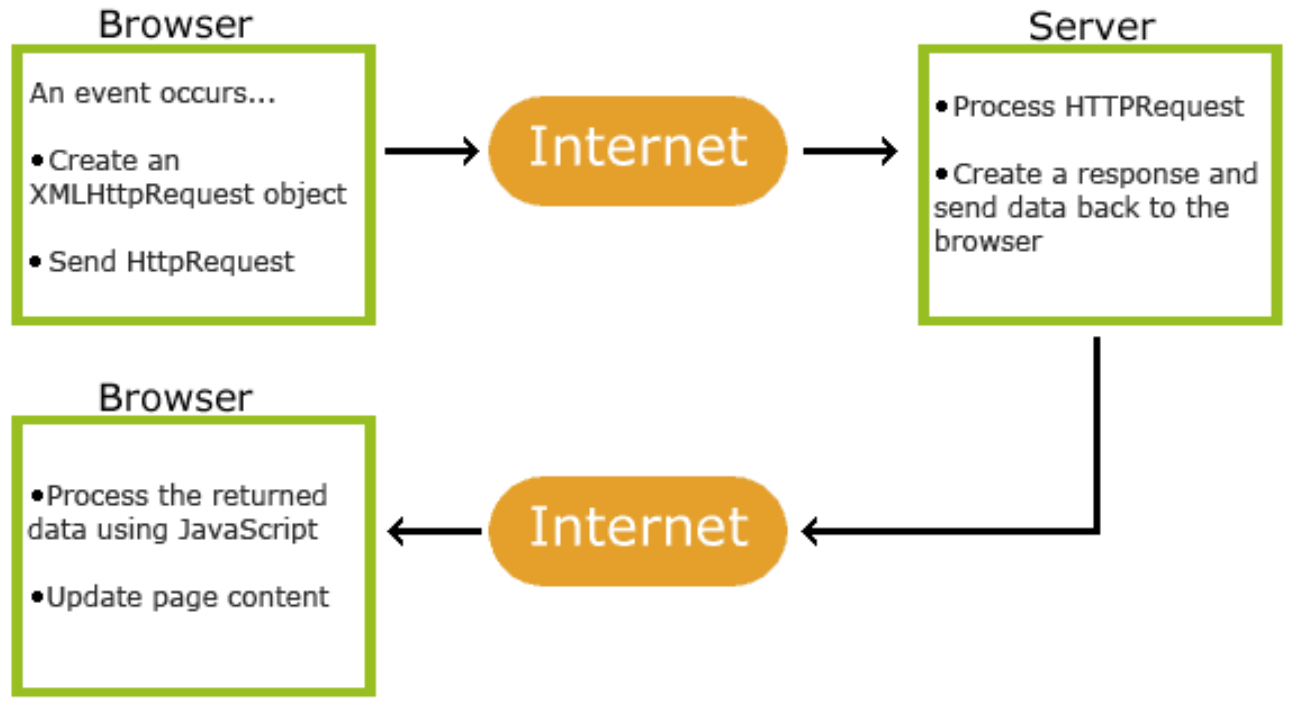
\includegraphics[width=0.7\textwidth]{ajax.png}
\end{center}

Код клиента в браузере, реагируя на какое-то событие (например клик по кнопке), создаёт объект XMLHttpRequest и подписывает коллбэк, который вызовется браузером, когда с сервера придёт ответ. Сам запрос --- это обычный HTTP-запрос, можно указать HTTP-метод, URL (относительно того места, откуда получена страница), и должен быть запрос асинхронным или нет (конечно да). Сервер получает запрос, формирует ответ и отправляет обратно --- как правило, в виде JSON-документа, потому что в JavaScript его даже десериализовывать не нужно, это сразу валидный объект. Браузер принимает ответ от сервера и исполняет коллбэк, который и обновляет содержимое (обычно, хотя может этого не делать). Вот пример:

\begin{minted}{html}
<!DOCTYPE html>
<html>
    <body>
        <div id="demo">
            <h2>The XMLHttpRequest Object</h2>
            <button type="button" onclick="loadDoc()">Change Content</button>
        </div>
        <script>
            function loadDoc() {
            var xhttp = new XMLHttpRequest();
                xhttp.onreadystatechange = function() {
                    if (this.readyState == 4 && this.status == 200) {
                        document.getElementById("demo").innerHTML = this.responseText;
                    }
                };
                xhttp.open("GET", "ajax_info.txt", true);
                xhttp.send();
            }
        </script>
    </body>
</html>
\end{minted}

Тут мы просто делаем на сервер GET-запрос для получения .txt-файла, после чего выставляем его содержимое (просто как текст) вместо кнопки, которая, собственно, и позволила его получить. Тут даже никакой содержательной логики на сервере писать не надо, любой веб-сервер (IIS, Apache) с обработкой такого запроса сам справится.

В какой-то момент (в стандарте ECMA 2017) в JavaScript добавили async/await, уже знакомые по C\# ключевые слова с очень похожей семантикой, так что коллбэки писать стало как-то не очень. Поэтому появился и более современный программный интерфейс для асинхронных запросов, опять-таки, встроенный в браузеры --- Fetch API. Он работает почти везде, кроме, конечно, Internet Explorer, а поскольку есть люди, которые им всё ещё пользуются, то к Fetch API всё ещё есть некое недоверие в сообществе. Зато это гораздо удобнее, гибче и мощнее XMLHttpRequest. Вот небольшой пример\footnote{На сей раз с developer.mozilla.org: \url{https://developer.mozilla.org/en-US/docs/Web/API/Fetch_API/Using_Fetch} (дата обращения: 18.11.2021).}:

\begin{minted}{javascript}
const data = { username: 'example' };

fetch('https://example.com/profile', {
  method: 'POST', // or 'PUT'
  headers: {
    'Content-Type': 'application/json',
  },
  body: JSON.stringify(data),
})
.then(response => response.json())
.then(data => {
  console.log('Success:', data);
})
.catch((error) => {
  console.error('Error:', error);
});
\end{minted}

Через Fetch API можно в принципе делать любые HTTP-запросы, даже файлы загружать (см. \url{https://developer.mozilla.org/en-US/docs/Web/API/Fetch_API/Using_Fetch} для примера).

\subsection{Промежуточное заключение}

Это необходимый минимум, чтобы писать хоть какие-то приложения с фронтендом, но на самом деле это отдельный большой мир, со своими языками, компиляторами/транспиляторами, системами сборки, огромным количеством библиотек, хороших и плохих практик, технических ограничений и т.д. Некоторая очень маленькая часть таких вещей будет рассмотрена в следующей лекции, но надо понимать, что это только вершина айсберга.

Кстати, всё, что мы делали до этого, не требует ничего, кроме браузера и любого текстового редактора. Строго говоря, даже сервера никакого не надо (если не хотите AJAX-запросы попробовать), браузер вполне может отрендерить просто файл .html и даже исполнять оттуда скрипты как ни в чём не бывало. Поэтому есть класс приложений, которые не имеют серверной части вообще и по сути представляют собой размещённые просто где-то .html-файлы со скриптами. Если задача это позволяет, так и надо делать, потому что их очень легко хостить --- <<статическое>> приложение (которое может быть очень даже динамическим, но не требует серверного бэкенда) можно разместить бесплатно, например, на GitHub Pages. Приложения, которым серверная часть хоть в каком-то виде нужна, требуют уже некоторого интеллекта для деплоя --- бесплатные хостинги для них существуют, но предоставляют смехотворное количество вычислительных ресурсов, да и выкладывание таких приложений гораздо более хлопотно.

\section{Бэкенд}

Теперь о том, что происходит на сервере. До того, как запрос попадает на обработку вашему коду, он обрабатывается сетевым стеком операционной системы, который вызывает веб-сервер, который \emph{хостит} ваше веб-приложение. Тут возможны две опции: веб-сервер запущен внутри процесса самого веб-приложения, либо веб-сервер отдельный (например, Internet Information Services, IIS) и веб-приложение работает внутри него (как плагин, фактически). Возможен и третий вариант --- когда веб-сервер работает как <<обратный прокси>>, перенаправляющий запросы на процесс веб-приложения, где работает его собственный веб-сервер.

Веб-сервер разбирает URL, на который пришёл запрос, понимает по нему, какому именно приложению он предназначается (если это не self-hosted-сервис, в этом случае и так всё понятно), и передаёт его на обработку \emph{веб-фреймворку}. Тот, в свою очередь, пропускает запрос через набор \emph{middleware}-обработчиков, которые могут выполнять разные преобразования, валидацию, логирование и т.д., и с помощью механизма \emph{роутинга} определяет, какой \emph{контроллер} и какой его метод должен обработать запрос. Определяет прежде всего по форме URL, а именно его части после доменного имени (например, \url{http://example.com/my/service} --- вызовется метод service контроллера my, ежели мы так захотим --- правила роутинга описываются разработчиком и могут быть, вообще говоря, какими угодно). В это же примерно время выполняется разбор параметров, которые передаются в URL или в теле запроса, так что метод контроллера получает уже готовые данные, как будто его вызвали, передав как параметры полноценные объекты. Контроллеры --- это уже код, который пишет автор приложения, они и являются точками входа в систему. Именно контролллер должен что-то сделать с запросом (обычно --- делегировать содержательную обработку классам бизнес-логики) и сформировать ответ, в виде либо какого-то сериализованного документа (если речь идёт про контроллер API), либо HTML-страницы (если контроллер отвечает на запрос браузера).

\subsection{ASP.NET, введение}

Всё, сказанное выше, относится к подавляющему большинству фреймворков по разработке веб-приложений, однако поскольку курс у нас на примере .NET, перейдём  к рассмотрению конкретно ASP.NET. ASP.NET разрабатывался как основное средство для написания веб-приложений под .NET, поэтому появился одновременно с самой платформой, в 2002 году, однако с тех пор был полностью переписан (возможно, неоднократно), сейчас называется ASP.NET Core, с открытым исходным кодом и распространяется под лицензией MIT. Старый ASP.NET доразвивался до версии 4.8 (работает только на .NET Framework, но до сих пор может встретиться в индустрии), затем версии сбросились и ASP.NET Core начался снова с версии 1.0. При этом, чтобы всех запутать, с переименованием .NET Core в просто .NET и прекращением развития .NET Framework ASP.NET Core переименовался просто в ASP.NET (но не везде --- Википедия, например, об этом не знает). К счастью, сейчас он версии 6, так что путаницы быть не должно.

ASP.NET предполагает несколько моделей разработки.

\begin{itemize}
    \item Многостраничные приложения --- где логика разделена на несколько страниц, по которым пользователь переходит, и которые генерируются на сервере. В таких приложениях клиентская часть обычно довольно минималистична, вся бизнес-логика реализуется на сервере, и часты полные перезагрузки страниц.
    \begin{itemize}
        \item Самый старый, громоздкий, но архитектурно правильный подход к разработке таких приложений --- ASP.NET MVC, когда приложение явно разделяется на \emph{модели} с кодом бизнес-логики, \emph{контроллеры}, отвечающие за роутинг и десериализацию сетевых запросов и вызов кода моделей, и \emph{виды}, отвечающие за генерацию HTML для клиента по данным, полученным от моделей. В ASP.NET за генерацию HTML в видах отвечает язык шаблонов Razor, где можно размечать HTML-документ кусками кода на C\#, которые генерят изменяемую часть HTML (на самом деле, очень многие фреймворки имеют какой-то шаблонный генератор, а язык PHP вообще построен на такой модели).
        \item Razor Pages --- упрощённая версия MVC, которая сейчас рекомендуется по умолчанию. Тут также есть виды, генерируемые с помощью Razor, но каждому виду соответствует своя бизнес-логика, которая объекдиняет в себе функциональность контроллера и модели (примерно как форма и code behind в библиотеках для создания оконных приложений).
        \item Server-side Blazor. Blazor --- это недавно появившаяся жутковатая технология для написания адекватной клиентской части на C\# (конечно, никому не нравистя программировать на JavaScript). Server-side Blazor-приложение генерирует на сервере HTML-ку, но не перезагружает её каждый раз по запросу, как делают два предыдущих метода, а открывает соединение с клиентом, куда динамически догружает изменившиеся части. Ни разу не пользовался, поэтому не могу сказать, насколько хорошо или плохо это работает.
    \end{itemize}
    \item Одностраничные приложения --- где клиент грузит страницу ровно один раз, и она динамически меняется при взаимодействии с пользователем, без перезагрузки. Всё взаимодействие с сервером выполняется асинхронно через AJAX-запросы и API серверной части.
    \begin{itemize}
        \item Традиционный подход к такой разработке --- использовать только контроллеры ASP.NET для создания веб-API серверной части и клиентские библиотеки JavaScript (например, Angular, React или Vue), чтобы его дёргать. Razor и вообще View-часть ASP.NET в этом случае не используется вовсе, вся генерация представления выполняется на клиенте прямо в браузере.
        \item Client-side Blazor --- ещё более новая и жуткая технология, которую только-только довели до продакшна. Код на C\# компилируется в Web Assembly и загружается на клиент как JavaScript-код, где и исполняется, иногда дёргая сервер асинхронными запросами. Это позволяет не учить JavaScript и всякие странные библиотеки, и не страдать от отсутствия нормального компилятора, при этом использовать любой код на .NET на клиенте, в том числе сторонние библиотеки, потому что ему всё равно, IL компилируется в JS. Кажется, что это отличная идея, но попытки реализовать такого рода трансляторы предпринимались с середины 2000-х (особенно в F\#-сообществе, потому что там любят трансляторы), и заканчивалось всё тем, что надо знать и .NET, и JavaScript (чтобы адекватно пользоваться API браузера и интегрироваться с существующим JavaScript-кодом), да ещё и работало это кривовато. Насколько хорош Client-side Blazor, опять-таки не знаю, поскольку ни разу им не пользовался.
    \end{itemize}
\end{itemize}

Мы начнём с многостраничных приложений, потому что они хорошо подходят, в общем-то, для большинства сценариев, легко превращаются в одностраничные при нужде, и существенно проще в написании. Однако надо понимать, что ASP.NET --- это один фреймворк, ему всё равно, какое приложение вы пишете, внутри всё работает одинаково (разве что Blazor несколько выбивается из общей архитектуры, но ему тоже нужны контроллеры). Любой вид приложения можно превратить в любой другой, просто перерасположив файлы внутри проекта --- различаются по сути только шаблоны при создании приложения и точки зрения на архитектуру.

\subsection{ASP.NET, архитектура}

Концептуально любое ASP.NET-приложение отображает входящие по сети запросы на исходящие, делая это с помощью промежуточного кода самого фреймворка (middleware) и пользовательского кода. В случае с подходом MVC всё устроено так:

\pagebreak

\begin{center}
    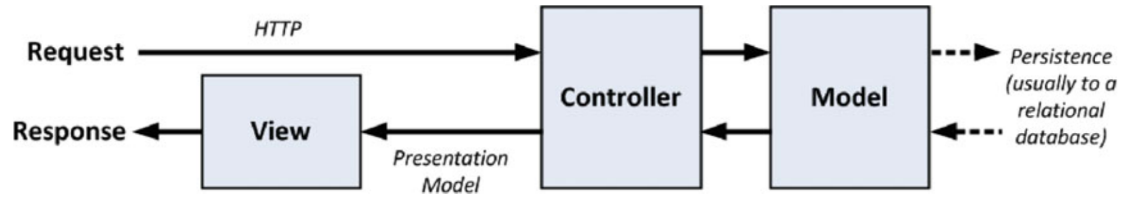
\includegraphics[width=0.7\textwidth]{mvc.png}
    \attribution{A. Freeman, Pro ASP.NET Core MVC}
\end{center}

\begin{itemize}
    \item \textbf{Модель} содержит или представляет данные, с которыми работает приложение, и бизнес-логику, которая делает с этими данными что-то полезное. При этом модель делится на две концептуаальные части.
    \begin{itemize}
        \item \textbf{Domain model} --- содержит объекты предметной области, включающие в себя бизнес-логику, и это единственное место в приложении, которое вправе содержать код, знающий, что это приложение делает и для чего оно нужно. Эта же часть общается с СУБД, чтобы где-то хранить свои данные (хотя вправе напрямую про СУБД ничего не знать, этим занимается Data Access Layer, который архитектурно не часть доменной модели, но про архитектуру попозже).
        \item \textbf{View Model} --- содержит классы, удобные для отображения во View, и предназначающиеся только для передачи информации между доменной моделью и клиентом.
    \end{itemize}
    \item \textbf{Представление} (View) отвечает за показ данных из модели пользователю. Это может быть неожиданно, но View работает на сервере, клиенту же передаётся только результат его исполнения (уже готовая HTML-ка). Она-то и отображается в браузере.
    \item \textbf{Контроллер} отвечает за роутинг и обработку входящих запросов, десериализацию переданных данных, координацию действий объектов доменной модели и формирование видов, которые надо отправить в ответ.
\end{itemize}

На рисунке выше не показано, что происходит, перед тем, как вызывается метод вашего контроллера. А на самом деле происходит много чего, что критически важно для работы приложения:

\begin{center}
    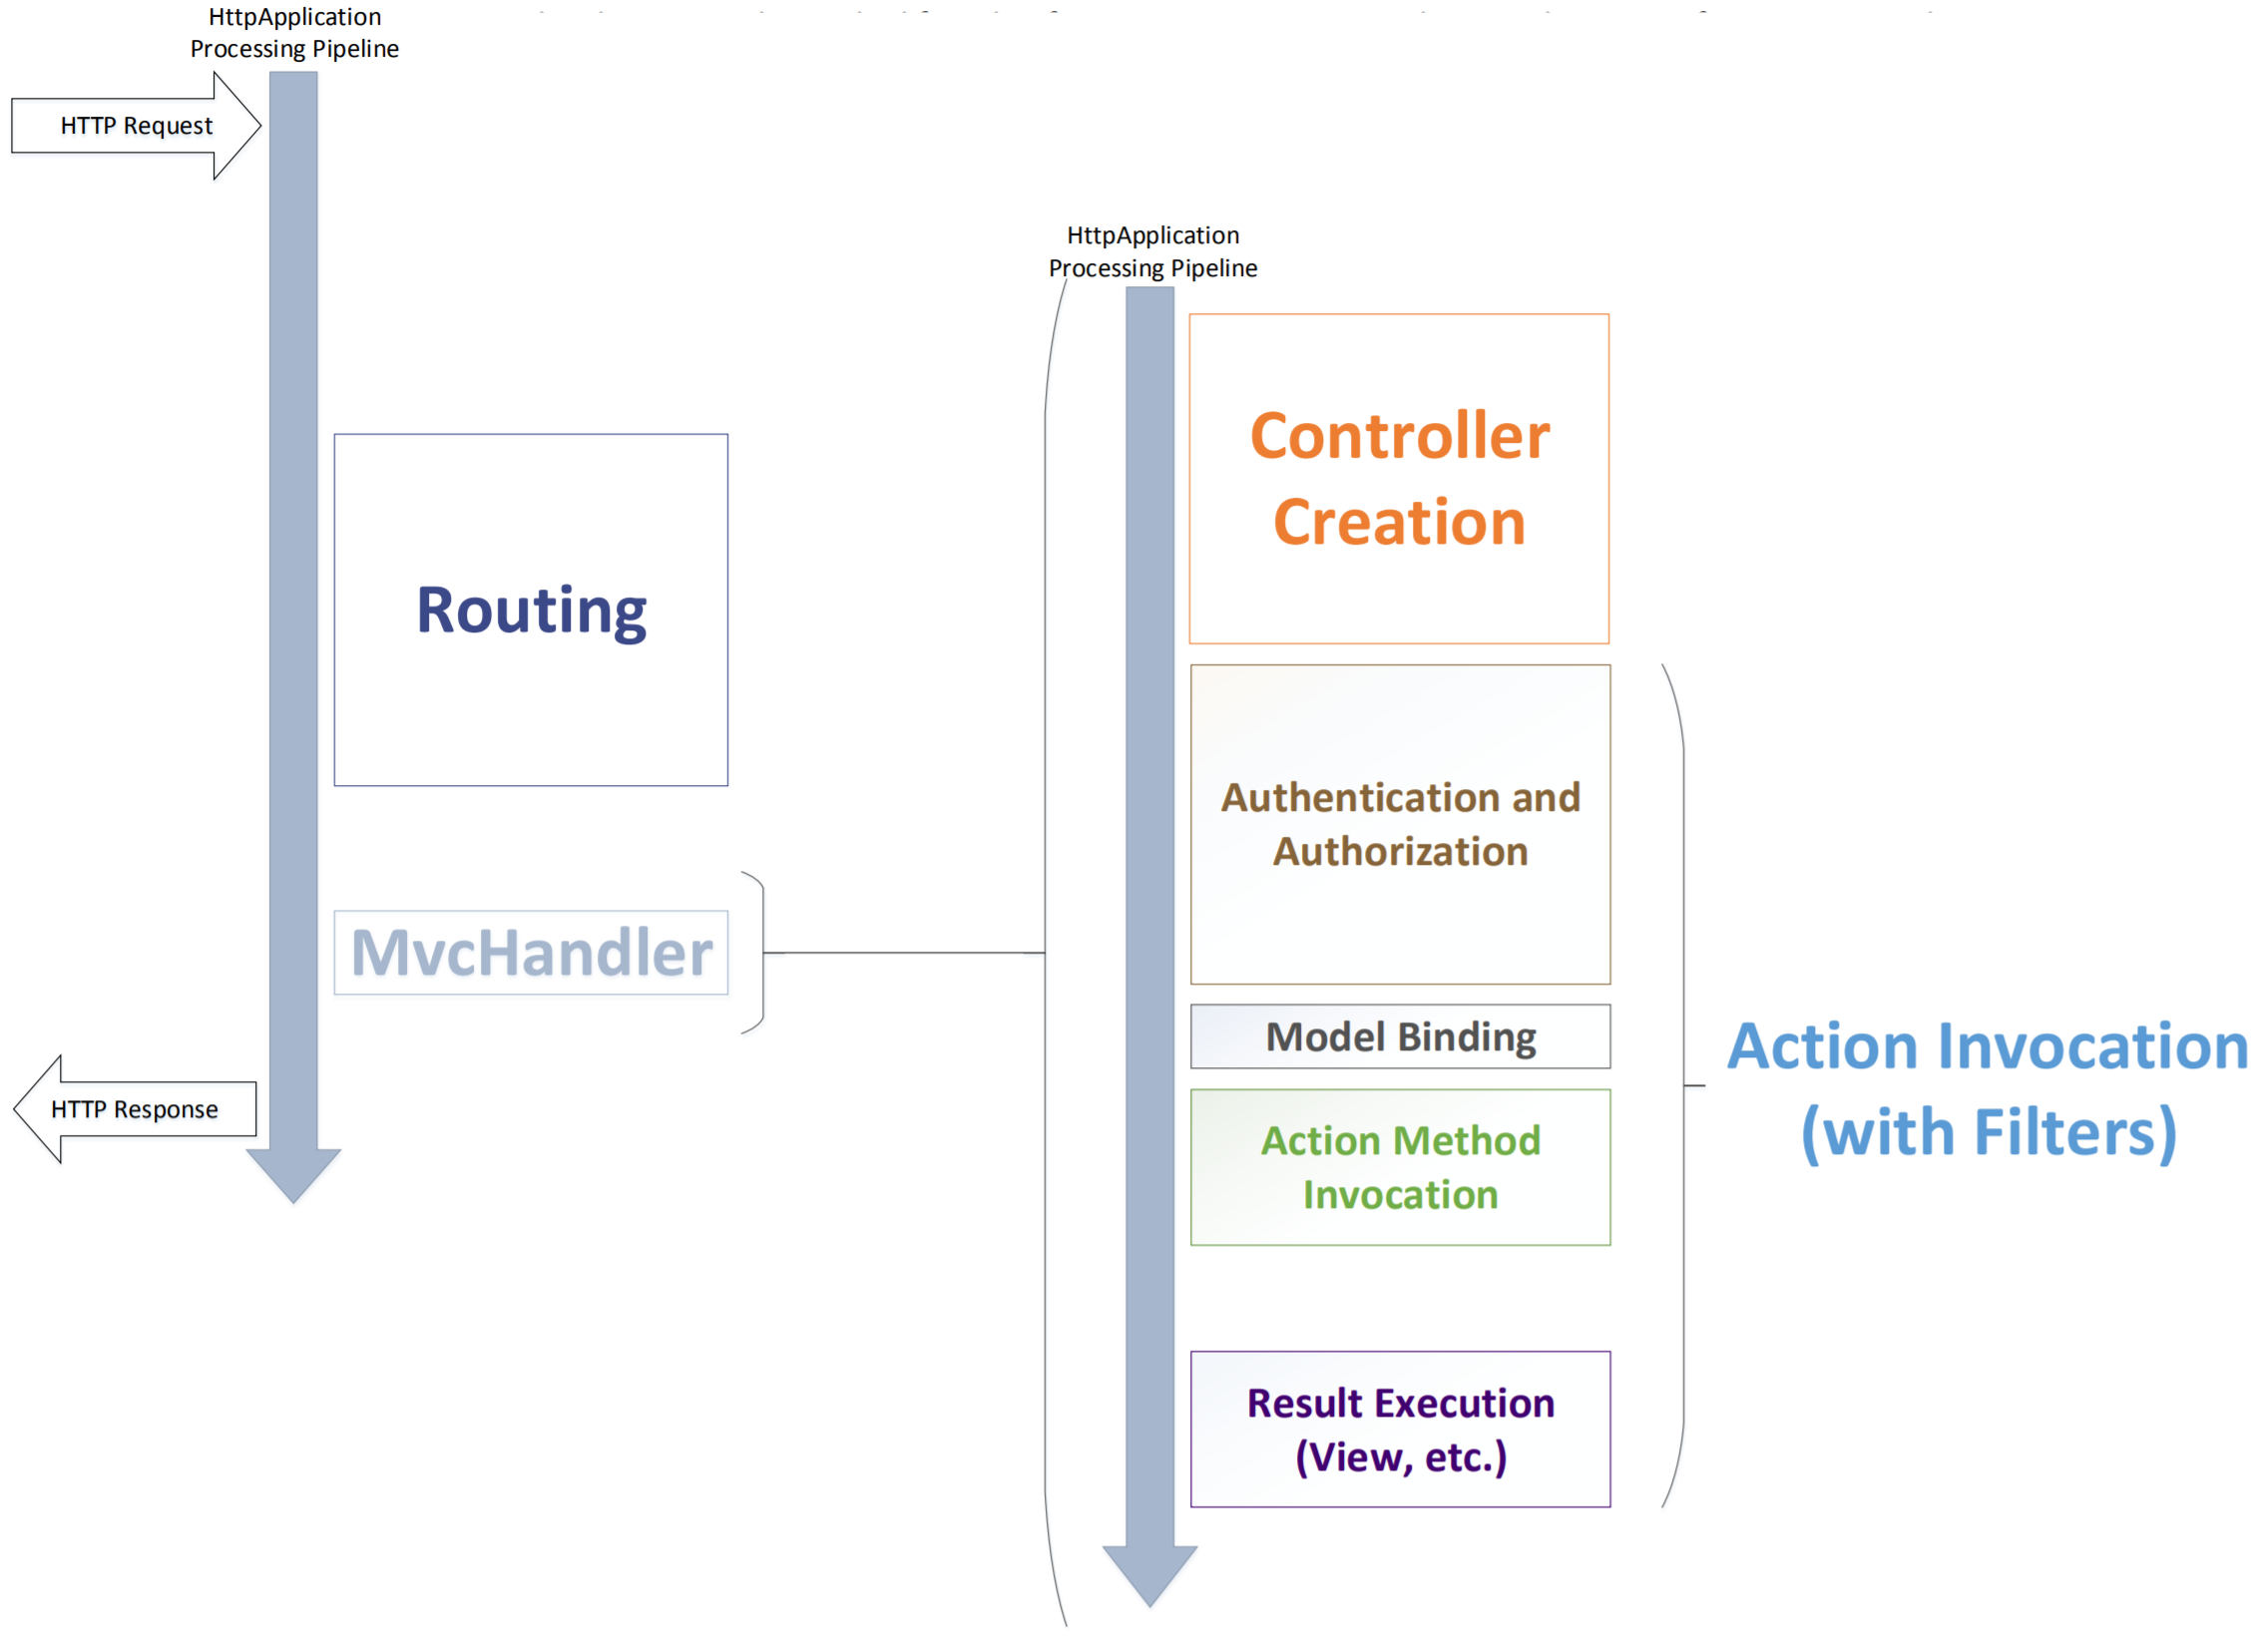
\includegraphics[width=0.85\textwidth]{requestLifecycle.png}
    \attribution{MSDN}
\end{center}

Входящий запрос принимается веб-сервером (например, Kestrel), который вызывает конвейер обработки запросов ASP.NET, который последовательно прогоняет запрос через следующие этапы:

\begin{itemize}
    \item роутинг --- по URL запроса понимаем, какой контроллер и какой метод контроллера надо вызвать, правила роутинга конфигурируются программистом либо через атрибуты у контроллеров, либо вручную из кода инициализации приложения;
    \item создание объекта контроллера, который должен обработать запрос;
    \item выполнение проверок аутентификации и авторизации для доступа к методам контроллера: если пользователь не аутентифицирован, вызывается обработчик ошибки, который, как правило, отправляет пользователя на страницу логина;
    \item \emph{model binding} --- парсинг запроса и отображение данных, пришедших в нём, на C\#-объекты, которые будут переданы методу контроллера при вызове;
    \item валидация модели --- если её указал программист, в виде атрибутов класса модели, проверка, что переданные данные соответствуют нашим пожеланиям (например, адрес электрононй почты, переданный нам при регистрации, подходит под соответствующий регэксп); невалидность модели, впрочем, не отменяет запуск метода контроллера, ему просто говорят, что модель невалидна;
    \item запускаются \emph{фильтры}, если они установлены --- например, чтобы сразу вернуть ошибку на клиент, если модель невалидна, не беспокоя контроллер;
    \item собственно вызов метода контроллера (который в ASP.NET вообще-то называется \emph{действием}, но поскольку это просто метод, не следует плодить термины без нужды);
    \item метод контроллера должен вернуть результат --- в большинстве случаев объект типа View, параметризованный view-моделью. Это на самом деле правило, по которому должна быть сгенерирована HTML-страница, и его надо исполнить. View пропускается через Razor, и на выходе, если всё хорошо, получается HTML. Она-то и отправляется обратно по HTTP браузеру как результат выполнения запроса.
\end{itemize}

На самом деле, любой из этих этапов конфигурируем и его можно полностью переопределить или добавить свои этапы, это всё конфигурируется при старте приложения. Однако в большинстве случаев стандартный конвейер делает своё дело и ничего трогать не надо.

\subsection{Структура проекта}

Теперь наконец можно попробовать это всё вживую. Если начать создавать в Visual Studio\footnote{Если вы пользуетесь чем-то ещё, не пугайтесь, dotnet new всё это тоже умеет.} веб-приложение, на выбор будет предложено несколько шаблонов: веб-приложение в формате MVC, веб-приложение Razor Pages, веб-API (<<обычный>> и на gRPC), два варианта Blazor (серверный и клиентский, как описывалось выше), три разных варианта SPA\footnote{Single-Page Application} с Angular и React, и пустое приложение, в которое при желании можно добавить всё, перечисленное выше, в любой пропорции, но вручную.

Если мы создадим MVC-приложение (оставив все настройки по умолчанию), получим работающее приложение, которое можно просто взять и запустить. Однако нас интересует структура проекта:

\begin{itemize}
    \item \textbf{wwwroot} --- статические ресурсы приложения (то, что можно включать в html-страницу), отправляются клиенту как есть. В подпапках css и js, думаю, понятно что лежит, в папке lib --- клиентские библиотеки (то есть те, что будут исполняться в браузере), по умолчанию добавленные к проекту. favicon.ico --- картинка, показывающаяся в заголовке вкладки браузера. Папка wwwroot доступна клиенту целиком и является той папкой, откуда отсчитываются относительные пути к ресурсам. Поэтому, в частности, не надо выкладывать туда все свои пароли или что-то такое.
    \item \textbf{Controllers} --- папка с, собственно, контроллерами. Их может быть несколько, и обычно либо один контроллер обслуживает одну страницу, либо контроллеры группируют логически связанную функциональность и обслуживают несколько страниц сразу. Поскольку ASP.NET использует принцип Convention-over-configuration, папку Controllers нельзя переименовывать или перекладывать куда-то, а все контроллеры должны иметь суффикс <<Controller>>, иначе придётся переконфигурировать роутинг (что несложно, но внезапная неработоспособность веб-приложения после одного маленького переименования может шокировать неопытного веб-программиста).
    \item \textbf{Models} --- папка с доменными и view-моделями, там можно завести подпапки и писать содержательный код, никакой ASP.NET-специфики в ней нет.
    \item \textbf{Views} --- папка с шаблонами HTML-страниц для представлений. Опять-таки, из-за Convention-over-configuration, Views должна называться именно так, и содержать в себе подпапки с именами, соответствующими именам контроллеров, которые возвращают эти вьюшки (например, Home для HomeController). Также там есть папка Shared, куда попадают вью, используемые несколькими контроллерами, и есть вью, шаблоны которых начинаются с подчёркивания. Это так называемые частичные представления, по сути куски шаблонов, которые сами по себе ничего хорошего не генерят, но могут использоваться в других шаблонах.
    \item \textbf{appsettings.json} --- конфигурация приложения. Сюда можно добавлять свои параметры конфигурации, а потом их читать (например, connection string к базе).
    \item \textbf{Program.cs} --- конфигурирует хост и запускает приложение. Здесь же конфигурируется роутинг, настраиваются обработчики ошибок, авторизация и прочие ужасные вещи, включая IoC-контейнер, используемый во всём приложении для получения <<глобальных>> вещей типа контекста базы данных и для конфигурирования внешних зависимостей.
\end{itemize}

Если же мы создадим приложение Razor Pages, то wwwroot, appsettings.json и Program.cs получатся тольно такими же, а вот вместо Controllers, Models и Views будет папка Pages, внешне похожая на папку Views из MVC. Однако под каждым .cshtml-файлом с шаблоном представления будет также лежать и .cs-файл (например, Index.cshtml.cs для Index.cshtml), который для данной страницы играет роль контроллера и обслуживает конкретно её. Такая структура проекта гораздо проще, потому что не нужно пытаться угадать, как надо назвать папку в Views, чтобы она совпала с каким-то из контроллеров, кроме того, заставляет контроллеры не разрастаться до невероятных размеров (что часто случалось с MVC). Поэтому подход с Razor Pages сейчас рекомендуемый.

\subsection{Razor}

Теперь поговорим подробнее о View-части. Как уже говорилось, представление в ASP.NET генерируется по шаблонам HTML-страниц, куда дописываются некие куски по данным, берущимся из ViewModel-ей. Генерацией занимается движок кодогенериции Razor.

Вообще Razor --- это продвинутый шаблонный генератор, который может использоваться для генерации чего угодно, хотя и <<заточен>> на генерацию веб-страниц. Razor поставляется с ASP.NET и завязан на его инфраструктуру, тем не менее есть stand-alone-версия, которая успешно использовалась нами для генерации кусков сайта кафедры, например.

Шаблон для Razor состоит из текста на целевом языке (в нашем случае HTML) и кода на C\#, который может выполнять какие-то полезные действия и генерировать HTML (или просто строки), которые вставляются в результирующем файле в то место, где этот код был написан. Причём это самый настоящий C\#, можно пользоваться классами из проекта, можно свои классы объявлять прямо в шаблоне, можно что угодно (и на самом деле, по шаблону просто генерится класс, где ваш код будет просто некоторыми его методами).

Razor исполняется на сервере --- это часто вызывает сложности, потому что он генерит HTML и относится к части приложения, относящейся к представлению. Так что из шаблона есть доступ ко всему, что знает сервер, но данные, отображаемые клиенту, будут актуальны только на момент генерации (например, если мы сгенерируем текущее время, клиенту отправится время на сервере). Из этого также следует, что сам шаблон клиент не увидит, он увидит только результат генерации --- поэтому, например, есть отдельно Razor-комментарии, которые нужны для комментирования шаблона и клиент их не увидит, и HTML-комментарии, которые являются частью шаблона и клиент сможет на них посмотреть, если откроет код страницы (опять-таки, не пишите туда ничего секретного).

\subsubsection{Синтаксис}

Синтаксис шаблона довольно простой:

\begin{itemize}
    \item HTML-разметка пишется как есть;
    \item код на C\# заключается в \verb|@{}|;
    \item если код состоит из одного оператора, достаточно только \verb|@|, скобки не нужны: например, \mintinline{csharp}{The time is @DateTime.Now}; оператором считается всё до первого пробела, за исключением операторов, про которые Razor знает, например, for;
    \item если код представляет собой выражение, которое возвращает значение, то его можно заключать в круглые скобки, опять-таки, без фигурных: \mintinline{csharp}{@(someValue * 10)};
\end{itemize}

Обратите внимание, что DateTime.Now в примере выше вызовется на сервере, так что это будет время на момент генерации страницы. Ещё некоторая тонкость заключается в том, что результат генерации не впечатывается напрямую в HTML, а пропускается через HttpServerUtility.HtmlEncode, что заставляет сгенерированную строку отображаться так, как она была сгенерирована, в браузере (например, если вы сгенерируете \mintinline{html}{<\body>}, то оно так и напечатаетмя у пользователя, а не закончит страницу). Если вы хотите, например, HTML-ные тэги генерировать, используйте Html.Raw (например, \mintinline{html}{@Html.Raw("<\body>")}).

Вот небольшой пример Razor-шаблона, генерирующего валидную HTML-ку:

\begin{minted}{csharp}
<h1>Cthulhu fhtagn!</h1>

@for (int i = 0; i < 300; ++i)
{
    <p>Cthulhu fhtagn!</p>
}
\end{minted}

Как видно, boilerplate-разметки, подсказывающей генератору, где код, а где HTML, почти нет (например, фигурная скобка --- это явно код на C\#, а перед ней нет собаки). Это потому, что Razor использует разные эвристики, чтобы это понять, и в большинстве случаев делает это вполне адекватно. Но именно что <<в большинстве случаев>>, поэтому ему надо иногда позсказывать. Правила отделения кода от HTML такие:

\begin{itemize}
    \item после \mintinline{text}|@| и до пробела (или до конца оператора) --- код; важное исключение --- параметры-типы генериков будут проинтерпретированы как HTML-тэг, так что если хотите их использовать, придётся ставить фигурные скобки;
    \item после открывающего тэга --- HTML-разметка;
    \item после \mintinline{text}|@:| --- HTML-разметка;
    \item \mintinline{text}|@* ... *@| --- комментарии (серверные, не отправляются клиенту);
    \item \mintinline{text}|@@| --- \mintinline{text}|@| в HTML (escaping);
\end{itemize}

\subsubsection{Хелперы}

В коде на C\# внутри Razor-шаблона могут встречаться так называемые \emph{хелперы} --- функции, которые генерируют HTML-код. Иногда довольно простые, типа Html.Raw, которую мы уже видели, иногда более хитрые:

\begin{itemize}
    \item Html.ActionLink --- генерирует ссылку на метод контроллера, например, \mintinline{csharp}{Html.ActionLink("About this Website", "About")} сгенерирует ссылку, по коику на которую пошлётся GET-запрос контроллеру About.
    \item Хелперы генерации HTML-форм: BeginForm, EndForm, CheckBox, TextBox, Password и т.д. Это всё можно писать и вручную, однако с хелперами может быть более читаемо, чем разбираться в разных сортах тэга input; тем более что хелперам можно указать, куда слать POST-запрос по нажатию на Submit.
\end{itemize}

Но самая интересная штука --- это TagHelper-ы. Это на самом деле произвольный код на C\#, который может генерировать HTML-разметку, но их использование выглядит как использование обычных HTML-тэгов:

\begin{minted}{html}
<img src="~/images/asplogo.png" asp-append-version="true">
\end{minted}

Это на самом деле не тэг img, а библиотечный тэг-хелпер Image, который автоматически дописывает хеш к имени изображения, так что в HTML-ку пойдёт вот такое:

\begin{minted}{html}
<img src="/images/asplogo.png?v=Kl_dqr9NVtnMdsM2MUg4qthUnWZm5T1fCEimBPWDNgM">
\end{minted}

Это нужно потому, что вообще картинки обычно кешируются, так что если вы обновили картинку на сервере, клиент её не увидит, а увидит старую из кеша. Проблема традиционно решалась тем, что на сервере вручную обновляли имя файла, чтобы кеш думал, что изображение новое. Однако это легко забыть, поэтому тэг-хелпер Image считает хеш файла (как git, но не уверен, что SHA-1, что впрочем, не важно) и дописывает его через <<?>> к имени файла (что никак не влияет на возвращаемый файл, но для кеша ссылки разные, следовательно, он затребует свежий файл с сервера).

Чтобы тег-хелперы работали, их надо явно импортировать в шаблон, Razor-директивой (да-да, есть и такие) @addTagHelper, например, \mintinline{text}{@addTagHelper *, Microsoft.AspNetCore.Mvc.TagHelpers}. Звёздочка тут означает, что надо импортировать все тэг-хелперы, через запятую идёт пространство имён, в котором они объявлены. ASP.NET имеет что-то около 20 тэг-хелперов в комплекте, и, конечно, можно писать свои.

\subsubsection{Модели}

Всё, описанное выше, не сильно полезнее статической HTML-страницы, поскольку пока что никак не параметризуется данными. В реальных приложениях данные берутся из классов доменной модели и передаются во View с помощью ViewModel-ов. Простой пример (на RazorPages):

\begin{minted}{html}
@page
@using RazorPagesIntro.Pages
@model IndexModel

<h2>Separate page model</h2>
<p>
    @Model.Message
</p>
\end{minted}

Директива @page тут говорит, что это Razor Page-страница, то есть она сама отвечает за свой роутинг и не требует контроллера (в этой же директиве при необходимости можно указать параметры роутинга, но про это чуть попозже). Директива @using --- это обычный using из C\# на самом деле, подключение пространства имён. Дальше @model --- директива, говорящая, что для этой страницы типом модели является C\#-класс IndexModel. Это на самом деле заставляет Razor в сгенерированном классе-генераторе (как бы бредово это ни звучало, но оно так работает --- по шаблону генерится класс на C\#, который уже в рантайме принимает модель и порождает HTML) сгенерировать свойство Model типа IndexModel, на которое потом можно ссылаться в шаблоне: @Model.Message делает именно это.

Теперь мы можем параметризовать генератор реальными данными:

\begin{minted}{csharp}
using Microsoft.AspNetCore.Mvc.RazorPages;
using System;

namespace RazorPagesIntro.Pages
{
    public class IndexModel : PageModel
    {
        public string Message { get; private set; } = "PageModel in C#";

        public void OnGet()
        {
            Message += $" Server time is { DateTime.Now }";
        }
    }
}
\end{minted}

Теперь при обращении к этой странице из браузера вызовется метод OnGet из этого code behind, который выставит Message в указанную строку, и после этого вызовется генератор, принимающий IndexModel в качестве Model-а. В реальной жизни модель может иметь свойства более сложных типов, да и заполняются они обычно как-нибудь более содержательно, но общая идея такая. 

В MVC-подходе контроллер возвращает объект View, принимающий модель в конструктор:

\begin{minted}{csharp}
public IActionResult Error()
{
    return View(new ErrorViewModel { 
        RequestId = Activity.Current?.Id ?? HttpContext.TraceIdentifier 
    });
}
\end{minted}

Но использует её точно так же, как и в режиме Razor Pages:

\begin{minted}{csharp}
@model ErrorViewModel

<h1 class="text-danger">Error.</h1>
<h2 class="text-danger">An error occurred while processing your request.</h2>

@if (Model?.ShowRequestId ?? false)
{
    <p>
        <strong>Request ID:</strong> <code>@Model?.RequestId</code>
    </p>
}
\end{minted}

MVC в этом плане архитектурно аккуратнее, поскольку позволяет описать ViewModel, отделённую от действий по обработке запросов и, как правило, очень простую, по одной на каждый View, поддерживаемый контроллером. Но это, естественно, сложнее, особенно с учётом того, что доменная модель ничего не должна знать про представления и напрямую классы доменной модели использовать в View --- дурной тон.

\subsection{Роутинг}

Роутинг --- базовая функциональность любого фреймворка для разработки веб-приложений, это определение того, кто должен обработать запрос, по виду URL. Конкретно в ASP.NET механизм роутинга определяет метод, который вызовется для обработки запроса. Роутинг в ASP.NET использует подход Convention over configuration, что очень удобно, если вы знаете, что происходит. Однако это совсем не дружественный к новичкам подход --- сначала всё работает как магия и вы не знаете, почему, потом вы что-то немного меняете и перестаёт работать всё вообще.

Итак, соглашения по умолчанию для Razor Pages-режима такие:

\begin{itemize}
    \item URL вида <<адрес сайта/>> или <<адрес сайта/Index>> отображаются в /Pages/Index.cshtml, которая должна называться именно так и лежать именно тут.
    \item /Pages/Contact.cshtml --- URL вида <<адрес сайта/Contact>>.
    \item /Pages/Store/Contact.cshtml --- <<адрес сайта/Store/Contact>>.
    \item /Pages/Store/Index.cshtml --- <<адрес сайта/Store>> или <<адрес сайта/Store/Index>>
\end{itemize}

Для MVC соглашения те же, но относительно имён контроллеров и методов. <<адрес сайта/>> ведёт на метод Index контроллера Home, <<адрес сайта/Contact>> --- на метод Contact контроллера Home, <<адрес сайта/Store/Contact>> --- на метод Contact контроллера Store, и думаю, что идея понятна.

Роутинг по умолчанию можно переопределить. В режиме Razor Pages это не то чтобы просто и не то чтобы поощряется (всё-таки весь смысл Razor Pages в простоте и детерминизме того, что когда вызывается), но можно:

\begin{minted}{csharp}
var builder = WebApplication.CreateBuilder(args);

// Add services to the container.
builder.Services.AddRazorPages(
    options => options.Conventions.AddPageRoute("/Index", "/Ololo"));
\end{minted}

Это добавляет роут вида <<имя сайта/Ololo>> для страницы Index (при этом старый роут всё ещё доступен). Пишется это дело в Program.cs. Если пострадать немного больше, можно настроить роуты немного более тонко, но это уже надо читать документацию.

В режиме MVC роутинг полностью под вашим управлением. Его можно конфигурировать глобально для всего приложения (и это рекомендуется, поскольку сразу видно, кто что обрабатывает). Делается это тоже в Program.cs, в частности, код из шаблона устанавливает роут по умолчанию:

\begin{minted}{csharp}
app.MapControllerRoute(
    name: "default",
    pattern: "{controller=Home}/{action=Index}/{id?}");
\end{minted}

Все URL входящих запросов (точнее, их части после слеша) проверяются на соответствие шаблону, и если указан контроллер и действие, вызывается соответствующий метод, если что-то не указано, подставляются умолчания (тут Home и Index). Можно добавить несколько разных роутов при желании. id? в конце говорит, что URL может иметь опциональный аргумент, например, <<адрес сайта/Store/Index/128>>, который может быть передан в контроллер как часть входных данных (про это чуть ниже, в разделе про Model Binding).

Можно указывать роуты у каждого контроллера или даже метода контроллера в виде атрибутов (что хуже глобального указания, но зато прямо в коде контроллера видно, как в него попасть):

\begin{minted}{csharp}
[Route("Ololo")]
public class HomeController : Controller
{
    [Route("")] // Прибавляется к роуту до контроллера, чтобы получилось /Ololo
    [Route("Ololo")] // Прибавляется к роуту, чтобы получилось "Ololo/Ololo"
    [Route("/")] // Никуда не прибавляется, определяет роут ""
    public IActionResult Index() {}
}
\end{minted}

Итого метод Index доступен аж по трём роутам в нашей системе.

Обратите внимание, что Razor Pages так вообще не умеет.

Кстати, GET- и POST-запросы с точки зрения роутов --- это разные вещи, и они обрабатываются разными методами. В Razor Pages у страницы есть обработчики OnGet и OnPost (и т.д. для остальных HTTP-методов), в MVC вид обрабатываемого запроса указывается в атрибуте метода\footnote{Подробности в MSDN, в частности, \url{https://docs.microsoft.com/en-us/aspnet/core/tutorials/first-mvc-app} (дата обращения: 20.11.2021).}:

\begin{minted}{csharp}
[HttpPost, ActionName("Delete")]
public async Task<IActionResult> DeleteConfirmed(int id)
{
    var movie = await _context.Movie.FindAsync(id);
    _context.Movie.Remove(movie);
    await _context.SaveChangesAsync();
    return RedirectToAction(nameof(Index));
}
\end{minted}

Этот метод вызовется по POST-запросу на URL, например, <<имя контроллера/Delete/5>>.

\subsection{Model binding}

Последняя пока ещё нерассмотренная часть конвейера обработки запроса --- это Model binding, то есть парсинг параметров запроса и конструирвоание по ним C\#-объектов, которые передаются как параметры вызванному действию. Рассмотрим, например, такой View на Razor Pages:

\begin{minted}{html}
@page
@model WebApplication1.Pages.IndexModel
@addTagHelper *, Microsoft.AspNetCore.Mvc.TagHelpers

<html>
<body>
    <p>
        Enter your name:
    </p>
    <form method="post">
        Name: <input type="text" name="name" />
        <input type="submit" />
    </form>
</body>
</html>
\end{minted}

Здесь создаётся HTML-форма с одним текстовым полем, и когда пользователь жмёт на submit, выполняется POST-запрос к code behind нашей страницы (на самом деле, POST тут не принципиален, аргументы можно передавать и в GET, просто для форм так принято). Значение, которое ввёл пользователь, можно получить аж тремя способами.

Первый, и самый популярный --- как параметр в методе-обработчике:

\begin{minted}{csharp}
namespace WebApplication1.Pages
{
    public class IndexModel : PageModel
    {
        public void OnGet()
        {

        }

        public void OnPost(string name)
        {
            Console.WriteLine(name);
        }
    }
}
\end{minted}

Второй, вручную, через свойство Request.Form класса PageModel, от которого наследуются классы-обработчики Razor Pages:  

\begin{minted}{csharp}
public void OnPost()
{
    var name = Request.Form["name"];
    Console.WriteLine(name);
}
\end{minted}

Третий --- через свойства класса-обработчика:

\begin{minted}{csharp}
[BindProperty]
public string Name { get; set; }

public void OnPost()
{
    Console.WriteLine(Name);
}
\end{minted}

Первый способ предпочтителен, однако если параметров много (например, вы принимаете POST-запрос с кучей разных данных), третий способ может быть лучше. Второй способ полезен для отладки, потому как если байндинг по параметрам не удастся, метод с нужными аргументами даже не вызовется, а тут хоть можно понять, что происходит и что нам пришло.

Удивительно то, что в MVC байндинг работает точно так же, только там ещё можно для метода контроллера указывать фрагмент роута и на что он должен забайндиться (пример с id выше). Таким образом можно байндить все нормальные примитивные типы и даже сложные типы, если у них есть конструктор без аргументов и свойства, в которые можно записывать. Даже коллекции можно байндить. Подробностей слишком много, чтобы про них тут рассказывать, поэтому отсылаем к первоисточнику: \url{https://docs.microsoft.com/en-us/aspnet/core/mvc/models/model-binding} (дата обращения: 20.11.2021).

\end{document}
